% Created 2023-01-14 sam. 22:20
% Intended LaTeX compiler: pdflatex
\documentclass[presentation]{beamer}
\usepackage[utf8]{inputenc}
\usepackage[T1]{fontenc}
\usepackage[french]{babel}
\usepackage[labelformat=empty]{caption}
\usepackage{verbatim}
\definecolor{purple_wada}{RGB}{128,71,189} %   #8047bdff
\definecolor{links}{HTML}{2A1B81}
\useoutertheme{infolines}
%
% Beamer options
%
\setbeamertemplate{caption}{\raggedright\insertcaption\par}
\setbeamercovered{transparent}
\setbeamertemplate{section in toc}[sections numbered]
\setbeamertemplate{subsection in toc}[square]
\setbeamertemplate{navigation symbols}{}
\setbeamercolor{section in head/foot}{bg=purple_wada, fg=white}
\setbeamercolor{subsection in head/foot}{bg=white, fg=purple_wada}
\setbeamercolor{title in head/foot}{fg=purple_wada,bg=white}
\setbeamercolor{author in head/foot}{fg=white,bg=purple_wada}
\setbeamercolor{date in head/foot}{fg=white,bg=purple_wada}
\setbeamercolor{frametitle}{fg=purple_wada,bg=white}
\setbeamercolor{block title}{fg=purple_wada,bg=white}
%
% Adding frame at each section
%
\AtBeginSubsection[]
{
\begin{frame}
\frametitle{Sommaire}
\tableofcontents[currentsection,currentsubsection]
\end{frame}
}
\usetheme{default}
\author{Doc. Malik Koné}
\date{\today}
\title{Cryptoéconomie}
\hypersetup{
 pdfauthor={Doc. Malik Koné},
 pdftitle={Cryptoéconomie},
 pdfkeywords={},
 pdfsubject={},
 pdfcreator={Emacs 28.2 (Org mode 9.4.6)}, 
 pdflang={French}}
\begin{document}

{
  \usebackgroundtemplate{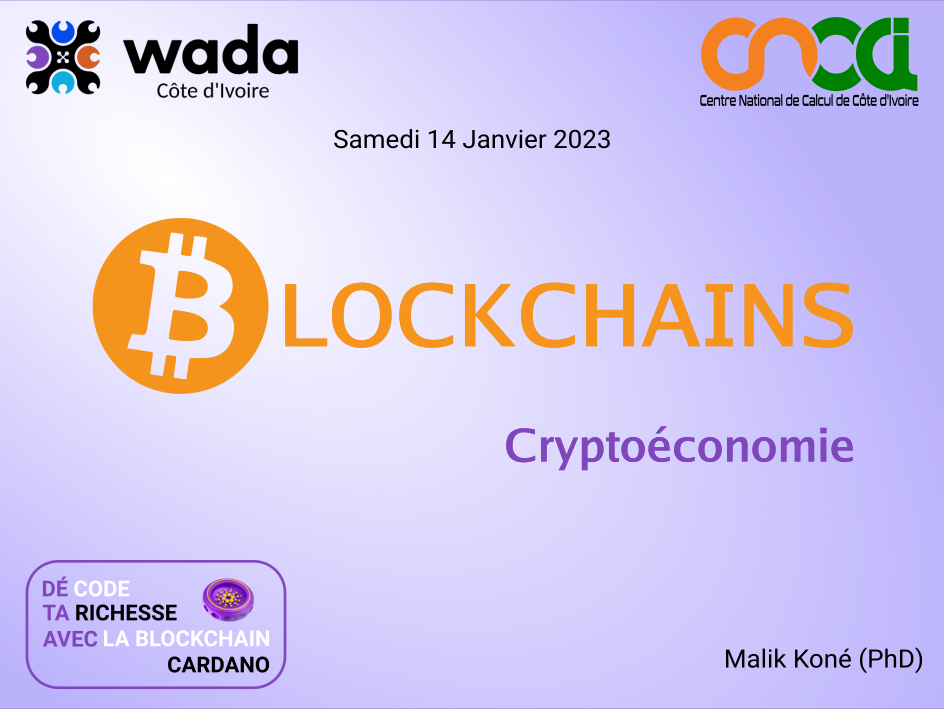
\includegraphics[height=\paperheight]{./page_de_garde_wadaci_j1b}}
  \frame[plain]{
  }
}

\section{Introduction}
\label{sec:org89be3d9}
\subsection{Notions de départ}
\label{sec:orgb0b1cbf}
\begin{frame}[label={sec:orgadae5c8}]{Notions de départ}
\begin{center}
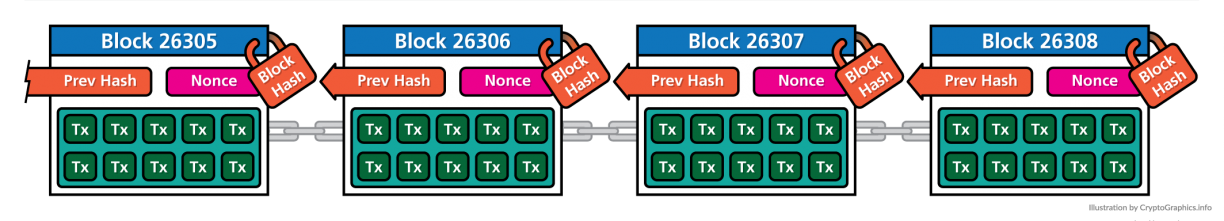
\includegraphics[width=\textwidth]{./Pictures/cryptographics/anatomy-of-a-chain-1.png}
\end{center}

\begin{columns}
\begin{column}{0.54\columnwidth}
\begin{block}<1->{Blockchain}
\begin{itemize}
\item <0>Décentralisation
\item <0>Consensus
\item <0>Cryptographie
\item <0>Applications décentralisées (dApp)
\end{itemize}
\end{block}
\end{column}
\begin{column}{0.46\columnwidth}
\begin{block}<1->{Cryptoéconomie}
\begin{itemize}
\item <2>Tokens ou jetons
\item <2>Marchés financiers
\item <2>Porte-monnaie de crypto (\href{https://yoroi-wallet.com}{Yoroi-wallet})
\end{itemize}
\end{block}
\end{column}
\end{columns}
\end{frame}

\subsection{La monnaie}
\label{sec:orgdb71ebd}
\begin{frame}[label={sec:orgee9bb31}]{}
\begin{verse}
Fiduciare, Scripturale, deviendrait-elle \alert{Crypturale} ?\\
\end{verse}
\end{frame}
\begin{frame}[label={sec:orgbc2cf2d}]{La monnaie}
\begin{columns}
\begin{column}{0.44\columnwidth}
\begin{block}{}
\begin{block}{Qu'est ce ?}
\only<1-6>{
\begin{itemize}
\item <1-5>Unité de valeur, de change et de compte
\item <5-6>Un jeu d'écriture
\end{itemize}
}
\end{block}

\begin{block}{Une histoire de confiance}
\only<8->{
\begin{itemize}
\item <8>L'obligation (autorité)
\item <8>La confiance (éthique)
\item <9-10>L'habitude (méthodique)
\end{itemize}
}
\end{block}
\end{block}
\end{column}
\begin{column}{0.55\columnwidth}
\begin{block}{}
\only<1>{
\begin{figure}[htbp]
\centering
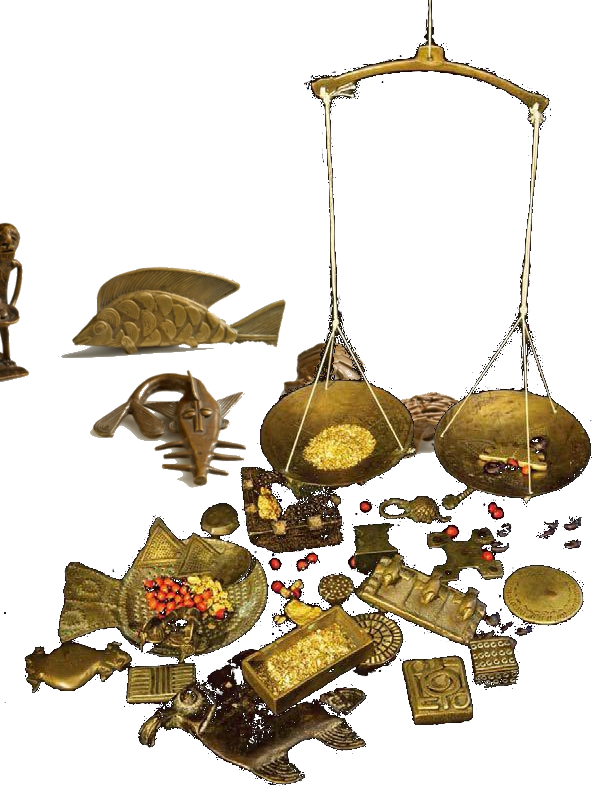
\includegraphics[width=.6\textwidth]{./Pictures/Cours2/poids_akan2.png}
\caption{poids Akan}
\end{figure}
}

\only<2>{
\begin{figure}[htbp]
\centering
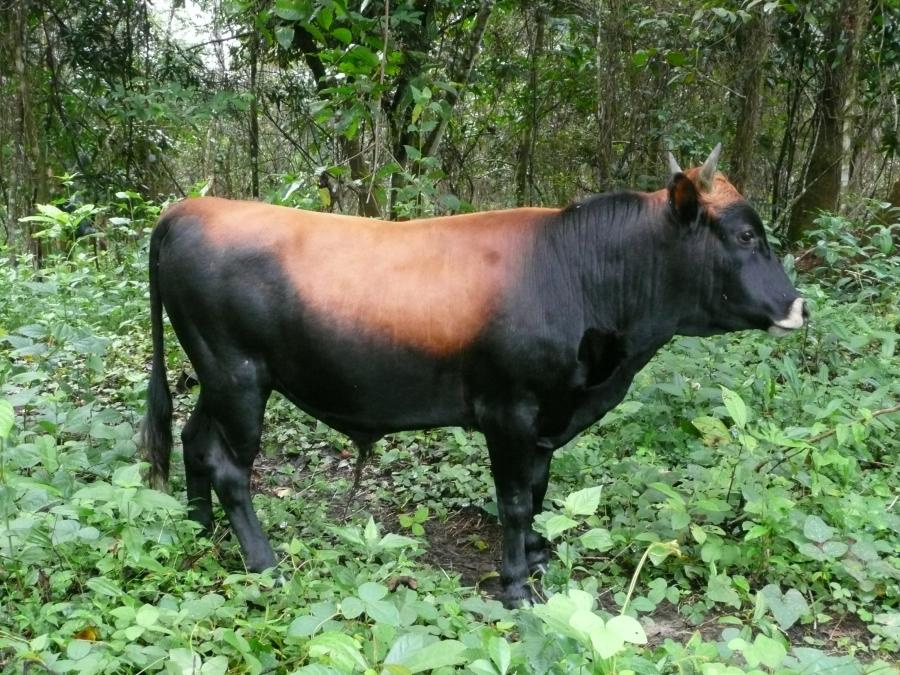
\includegraphics[width=.9\textwidth]{./Pictures/Cours2/pecu.jpeg}
\caption{pecu}
\end{figure}
}

\only<3>{
\begin{figure}[htbp]
\centering
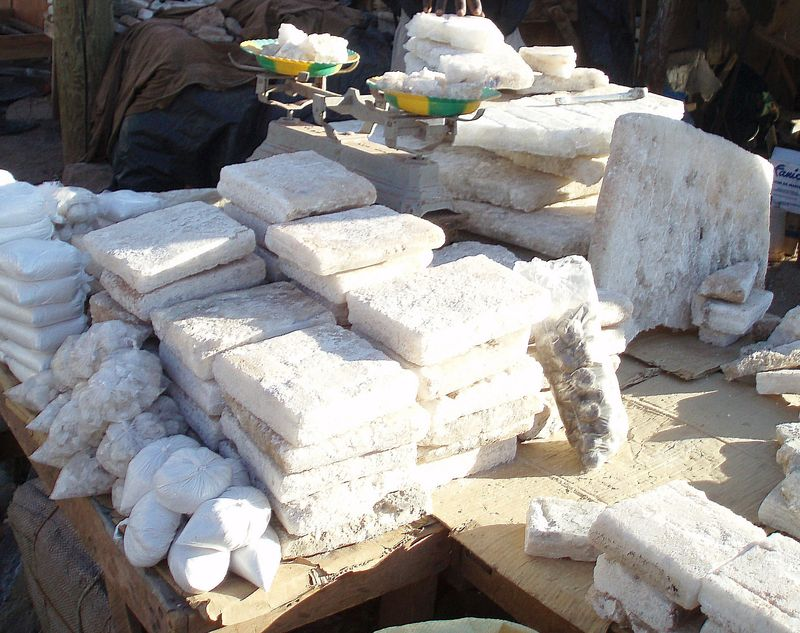
\includegraphics[width=.9\textwidth]{./Pictures/Cours2/sel.jpg}
\caption{barres de sel}
\end{figure}
}

\only<4>{
\begin{figure}[htbp]
\centering
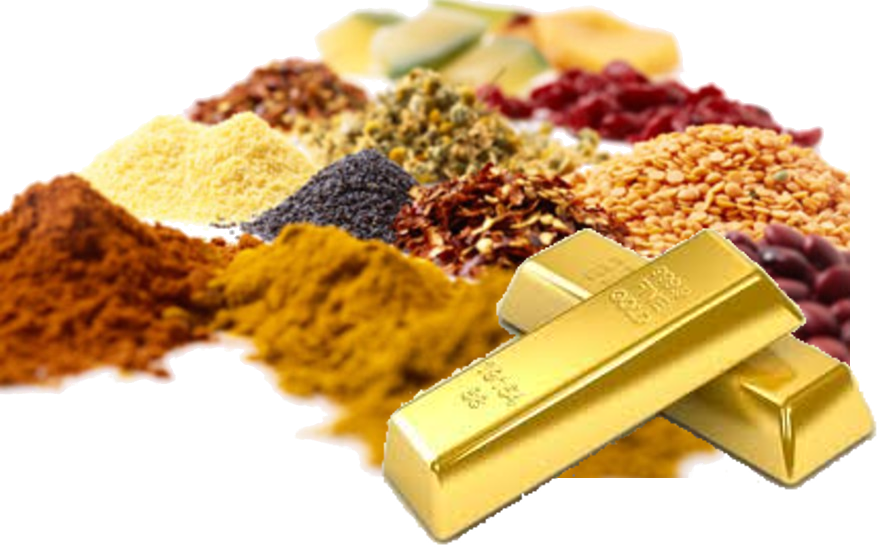
\includegraphics[width=.9\textwidth]{./Pictures/Cours2/epices_or.png}
\caption{épices et pièces}
\end{figure}
}

\only<5>{
\begin{figure}[htbp]
\centering
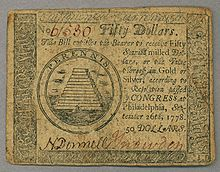
\includegraphics[width=.9\textwidth]{./Pictures/continental_note.png}
\caption{billet de 1778}
\end{figure}
}

\only<6>{
  \begin{figure}[htbp]
\centering
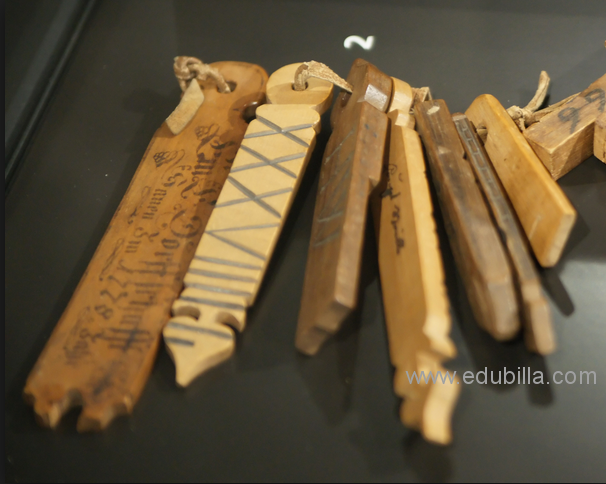
\includegraphics[width=.9\textwidth]{./Pictures/Cours2/tallystick3.png}
\caption{tally-stick, stocks \& foil}
\end{figure}
}    

\only<7>{
\begin{figure}[htbp]
\centering
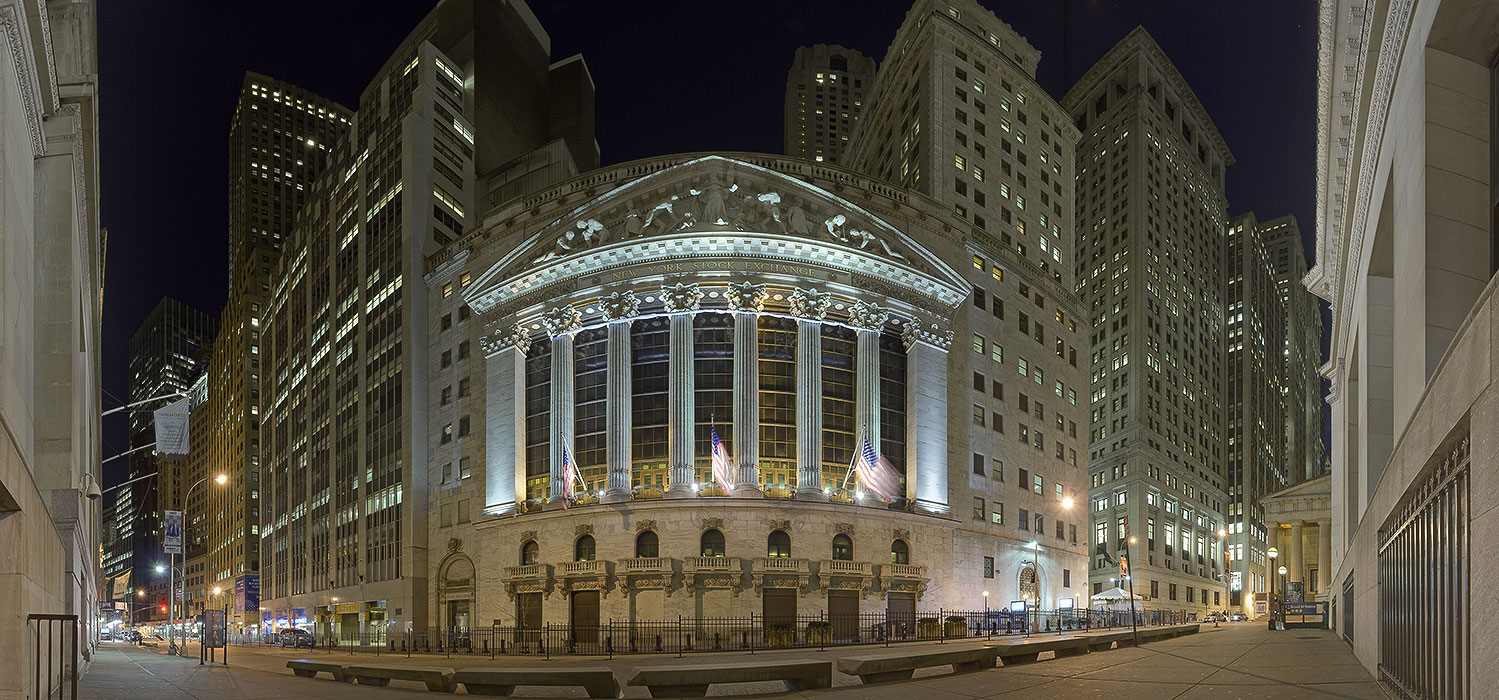
\includegraphics[width=.9\textwidth]{./Pictures/Cours2/wallstreet_stock.jpeg}
\caption{Wall-street ou le \emph{stock-exchange}}
\end{figure}
\begin{itemize}
     \item valeur légale
     \item presque entièrement digitalisée
\end{itemize}
}

\only<8>{
\begin{figure}[htbp]
\centering
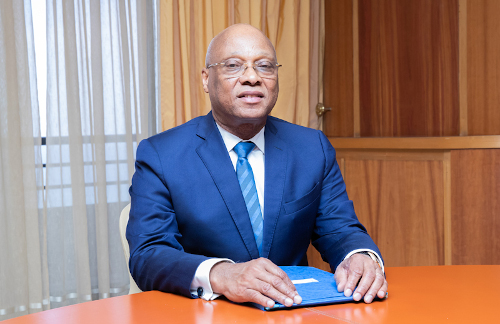
\includegraphics[width=.9\textwidth]{./Pictures/GouverneurBCEAO_Jean_Claude_BROU.jpg}
\caption{M. Jean-Claude Kassi Brou}
\end{figure}
}
\only<9>{
  \begin{center}
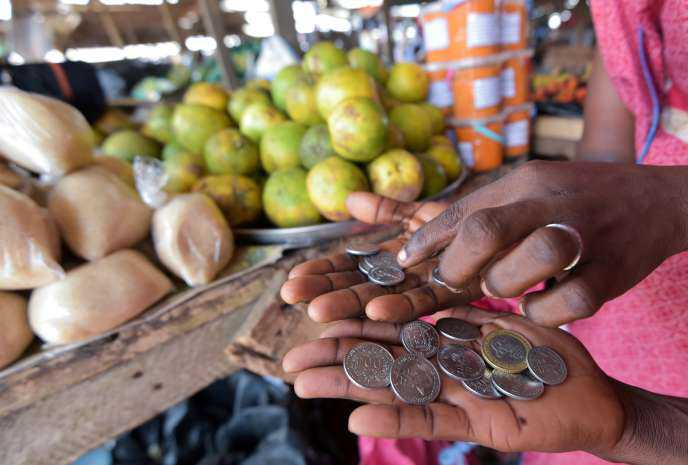
\includegraphics[width=.9\textwidth]{./Pictures/piece.jpg}
\end{center}
  }
\only<10>{
\begin{figure}[htbp]
\centering
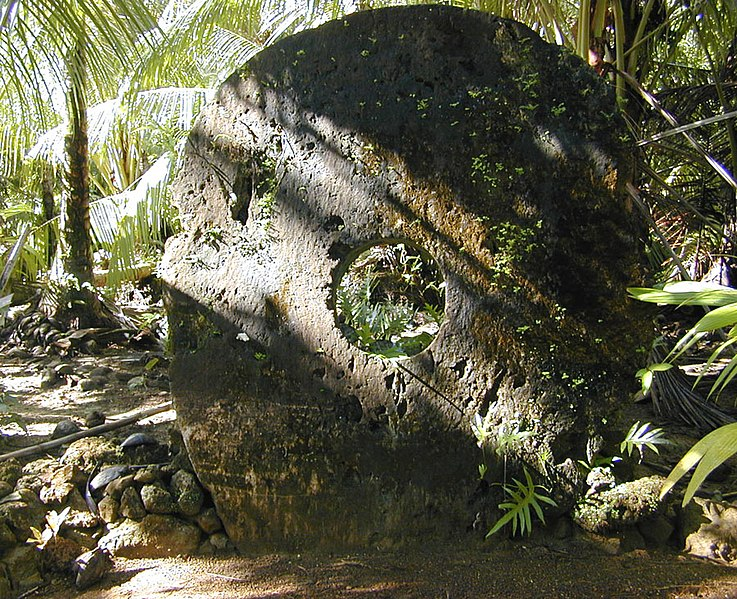
\includegraphics[width=.9\textwidth]{./Pictures/yap_Stone_Money.jpg}
\caption{sur les îles de Yap}
\end{figure}
}
\end{block}
\end{column}
\end{columns}
\end{frame}

\section{Token ou cryptoéconomie}
\label{sec:org61dea7e}
\subsection{Que sont les  cryptomonnaies ?}
\label{sec:orgae42cca}
\begin{frame}[label={sec:org4728df8}]{C'est comme des jetons de baby-foot, des unités téléphoniques ou des points de fidélité}
\begin{columns}
\begin{column}{0.38\columnwidth}
\begin{block}{}
\only<1-2>{
\alert{Mais} : 
\begin{itemize}
\item <2> pas de faussaires
\item <2> pas d'intermédiaires
\item <2> pas d'obligation d'usage
\end{itemize}
}
\end{block}
\end{column}
\begin{column}{0.38\columnwidth}
\begin{block}<1-2>{}
\begin{center}

\includegraphics[width=\textwidth]{./Pictures/arcade_token.png}
\end{center}
\end{block}
\end{column}
\end{columns}
\end{frame}

\begin{frame}<3-5>[label={sec:org38fa41b}]{Leurs usages}
\begin{columns}
\begin{column}{0.43\columnwidth}
\begin{block}{}
\begin{itemize}
\item <3->protocolaire
\item <4->applicatifs (dont NFT)
\item <5->gouvernance
\end{itemize}
\end{block}
\end{column}
\begin{column}{0.43\columnwidth}
\begin{block}<2-5>{}
\only<3>{
\begin{center}

\includegraphics[width=.9\textwidth]{./Pictures/logos/tokens_protocolaires.png}
\end{center}
}
\only<4>{
\begin{figure}[htbp]
\centering
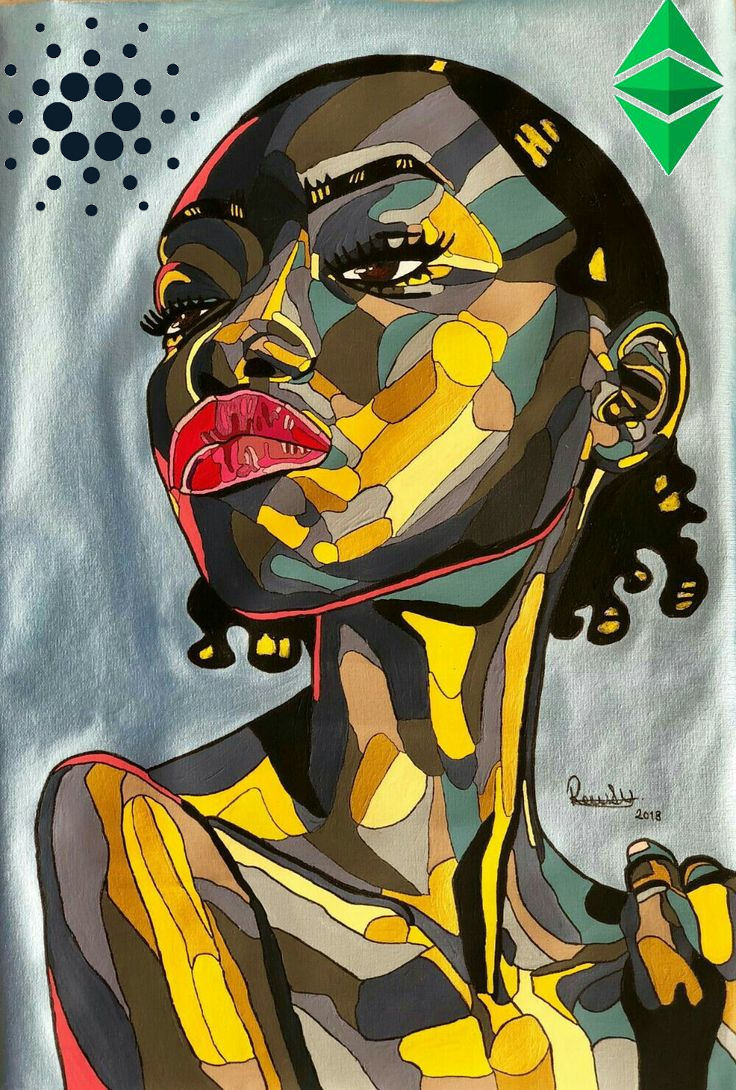
\includegraphics[width=.8\textwidth]{./Pictures/logos/tokens_applicatifs.png}
\caption{\emph{Non Fongible Token} (NFT)}
\end{figure}
}
\only<5>{
\begin{center}

\includegraphics[width=.9\textwidth]{./Pictures/logos/gouv_token.png}
\end{center}
}
\end{block}
\end{column}
\end{columns}
\end{frame}

\begin{frame}<6>[label={sec:org5707b15}]{Leur fonctions}
\begin{block}{}
Unités de compte, réserves de valeur, intermédiaires dans les échanges
\end{block}
\begin{block}<6>{}
\begin{center}
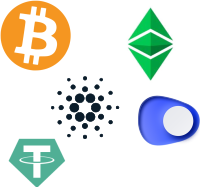
\includegraphics[width=.5\textwidth]{./Pictures/logos/tokens_tous.png}
\end{center}
\end{block}
\end{frame}


\subsection{Cryptomonnaie par la pratique}
\label{sec:org0f2e54d}
\begin{frame}[label={sec:org4fc68da}]{Comment obtenir des crytpomonnaies Aujourd'hui?}
\begin{block}{}
\begin{itemize}
\item \href{https://bitcoin.fr/acheter-bitcoin/}{Marchés en ligne}
\item Parainnages et programmes d’affiliations
\item Miner des bitcoins
\item Vendre de biens ou des services en Bitcoin (voir la \href{https://coinmap.org/view/\#/world/32.99023556/10.98632813/4}{carte})
\end{itemize}
\end{block}
\begin{block}{Attention}
\alert{Si c'est gratuit}, \emph{c'est probablement vous la marchandise}
\end{block}
\end{frame}

\begin{frame}[label={sec:org5c05b09}]{Qu'est-ce qu'un porte-monnaie de Bitcoins}
\begin{block}{voir la  \href{https://www.youtube.com/watch?v=oTfOfqmb5tU\&feature=emb\_err\_woyt}{Vidéo}}
\begin{center}
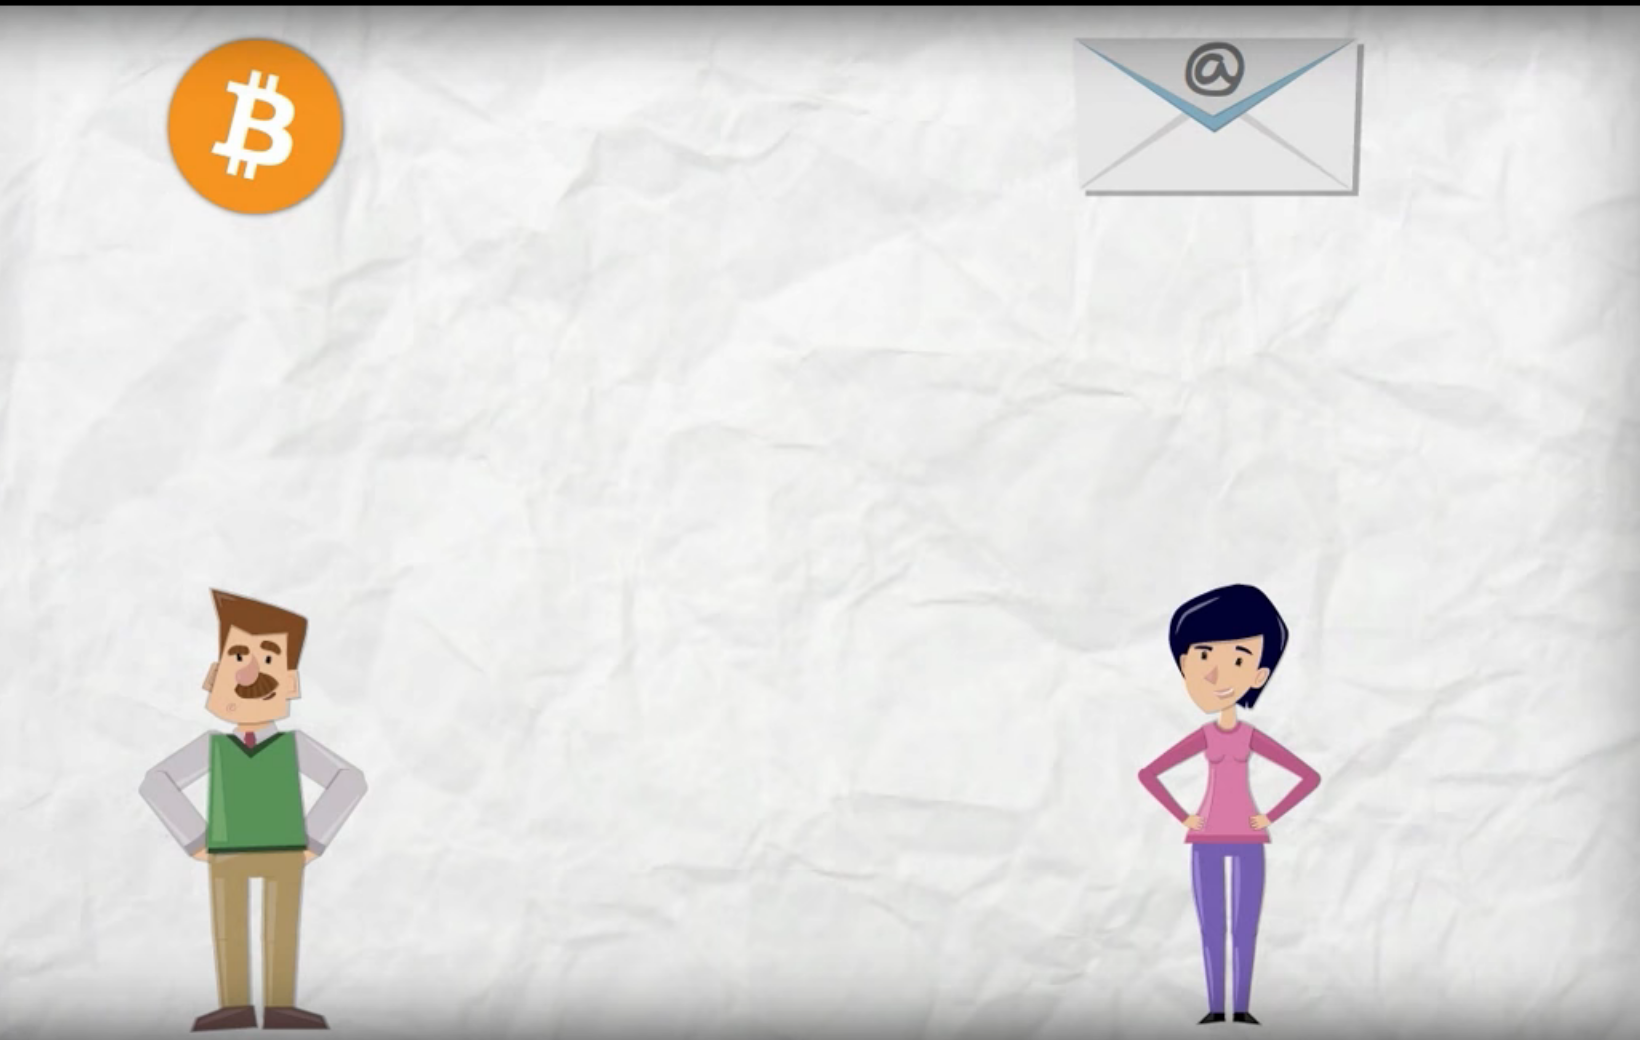
\includegraphics[width=.9\textwidth]{./Pictures/Cours2/wallet.png}
\end{center}
\end{block}
\end{frame}

\begin{frame}[label={sec:orgd5fe886}]{Comment conserver ses cryptomonnaies ?}
\begin{block}{\alert{Au frais / Cold Wallets}}
\begin{columns}
\begin{column}{0.50\columnwidth}
\begin{block}{noeud complet}
\begin{center}
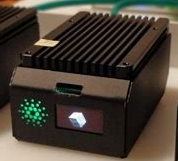
\includegraphics[width=.25\linewidth]{./Pictures/cardano/node.png}
\end{center}
\end{block}
\end{column}

\begin{column}{0.50\columnwidth}
\begin{block}{porte-monnaie matériel}
\begin{center}
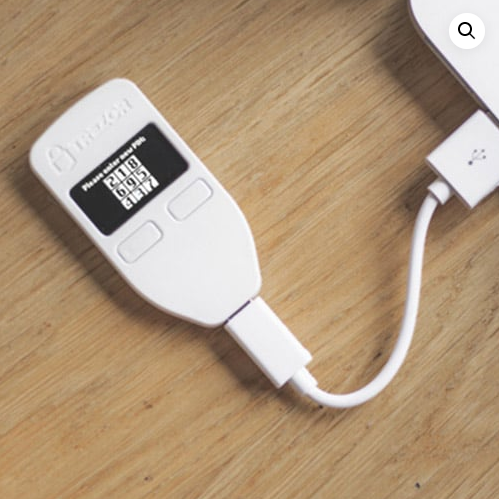
\includegraphics[width=.25\linewidth]{./Pictures/wallet_trezor.png}
\end{center}
\end{block}
\end{column}
\end{columns}
\end{block}

\begin{block}{\alert{Au chaud / hot Wallets}}
\begin{columns}
\begin{column}{0.50\columnwidth}
\begin{block}{porte-monnaie léger (Yoroi)}
\begin{center}
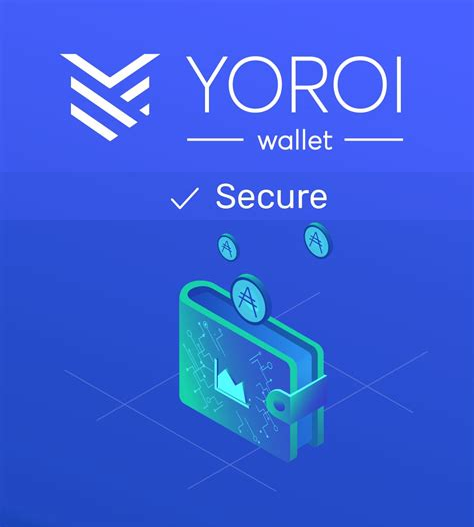
\includegraphics[width=.25\linewidth]{./Pictures/cardano/yoroi-small.png}
\end{center}
\end{block}
\end{column}

\begin{column}{0.50\columnwidth}
\begin{block}{Coinbase, Kraken, Binance}
\begin{center}

\includegraphics[width=.3\linewidth]{./Pictures/logos/logos_exchanges.png}
\end{center}
\end{block}
\end{column}
\end{columns}
\end{block}
\end{frame}

\begin{frame}[label={sec:org62f7417}]{Exemple d'un achat en Bitcoin}
\href{//youtu.be/hsuwxrB6c-M?t=82}{Paiement au El-Salvador en un éclair} (avec le réseau \emph{lighting})
\begin{center}
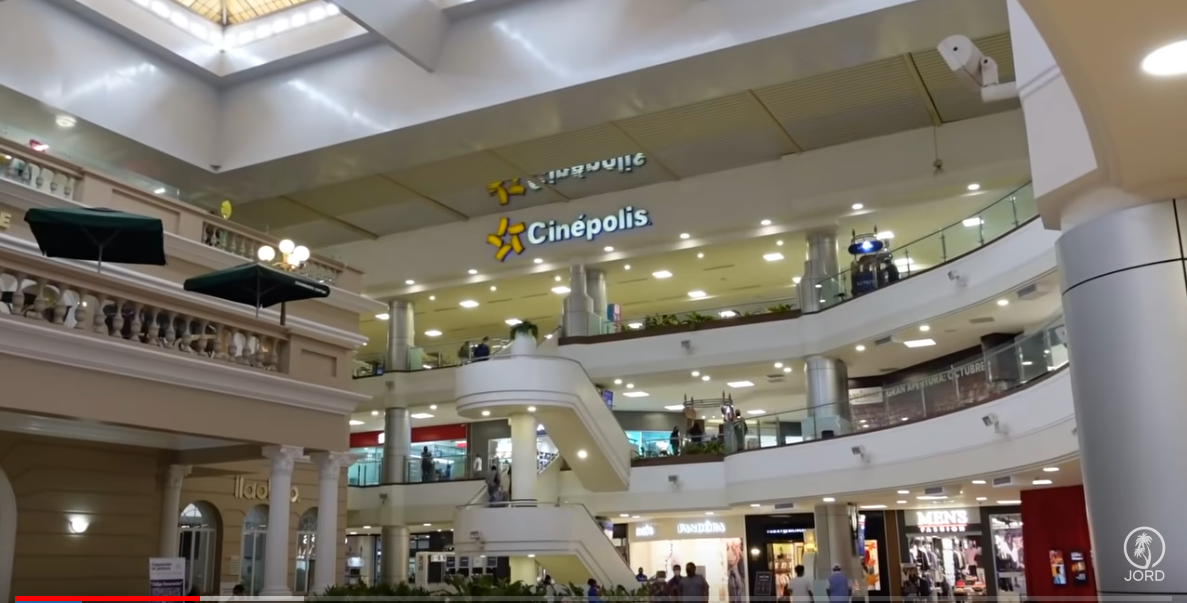
\includegraphics[width=.9\linewidth]{./Pictures/achat_lightning.png}
\end{center}
\end{frame}

\subsection{Le marché des cryptomonnaies}
\label{sec:org2a88793}
\begin{frame}[label={sec:org2c86b16}]{Le marché des cryptomonnaies}
\begin{center}
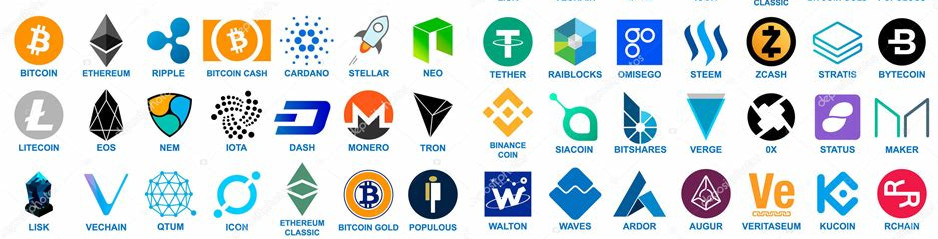
\includegraphics[width=.9\linewidth]{./Pictures/logos/cryptos.jpeg}
\end{center}

\begin{columns}
\begin{column}{0.4\columnwidth}
\begin{block}<2->{Dizaines de milliers de /coins/*}
\begin{itemize}
\item <2>memes coins
\item <2>stable coins
\item <2>shit coins
\end{itemize}

\only<3>{\tiny{
ref. \href{https://coingecko.com}{coingecko} et \href{https://coinmarketcap.com}{coinmarketcap}
}}
\end{block}
\end{column}

\begin{column}{0.6\columnwidth}
\begin{block}<3->{Marchés des cryptomonnaies}
\begin{itemize}
\item les crédits: \$~250~billions
\item Les actions: \$~80~billions
\item l'or: \$~7~billions
\item \alert{les cryptos: \$~1~billion}
\end{itemize}
\end{block}
\end{column}
\end{columns}
\end{frame}

\section{Perspectives}
\label{sec:org632896f}
\subsection{Perspectives}
\label{sec:orgcebbb15}
\begin{frame}[label={sec:org525fd72}]{Ceci n'est pas un cours de trading ?}
\begin{columns}
\begin{column}{0.57\columnwidth}
\begin{block}<1>{}
\begin{figure}[htbp]
\centering
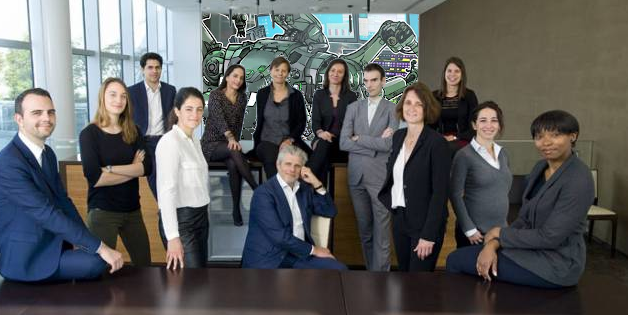
\includegraphics[width=\linewidth]{./Pictures/trading_team.png}
\caption{Des experts et \ldots{}}
\end{figure}
\end{block}
\end{column}

\begin{column}{0.42\columnwidth}
\begin{block}{}
\begin{figure}[htbp]
\centering
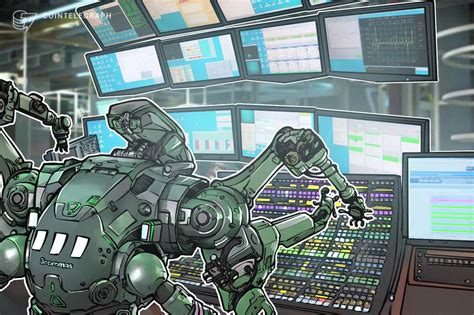
\includegraphics[width=\linewidth]{./Pictures/pro_bot.jpeg}
\caption{des bots, des IA, \textbf{de guerre}}
\end{figure}
\end{block}
\end{column}
\end{columns}
\end{frame}
\begin{frame}[label={sec:org1b40a03}]{Mais vous pourrez vous défendre (voir passer à l'attaque ?)}
\end{frame}
\end{document}